\chapter{Исследовательская часть}

\section{Сравнение результатов затенения}
На рисунках \ref{img:rsm}--\ref{img:fong} представлены результаты
визуализации с использованием различных методов затенения.
Причём была использована одна и та же сцена с одинаковым освещением.
Затухание света с расстоянием до источника не учитывалось.
Коэффициенты пропускания зелёного и розового объектов равны $0.1$ и $0.3$
соответственно, коэффициенты отражения -- $0.3$ и $0.4$ соответственно,
а диффузного отражения -- $0.6$ и $0.3$ соответственно.

\begin{figure}[H]
	\centering
	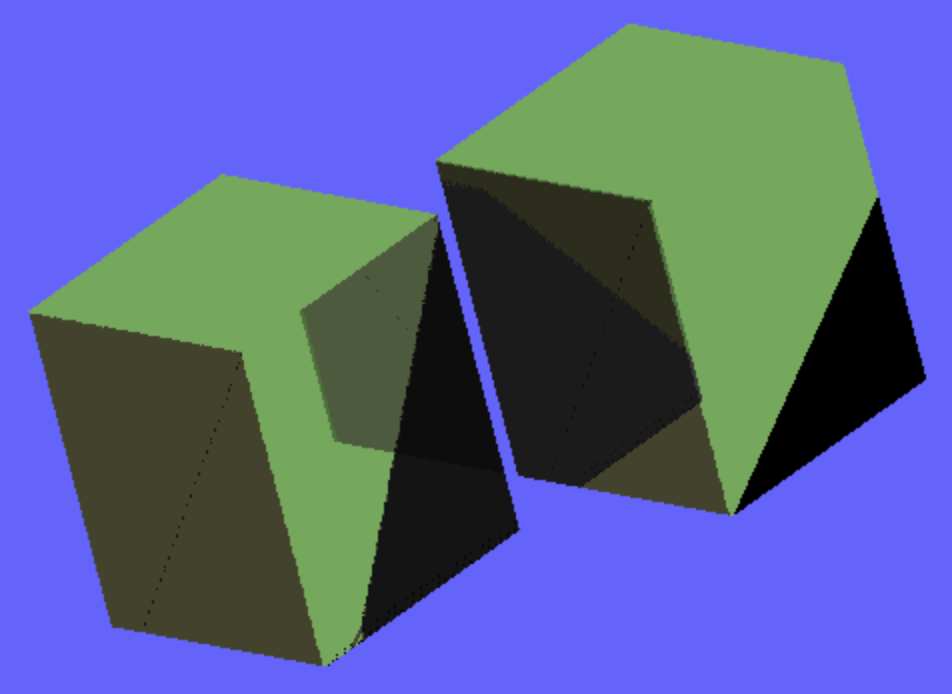
\includegraphics[width=0.5\textwidth]{img/rsm.png}
	\caption{Затенение с помощью карты теней.}
	\label{img:rsm}
\end{figure}

\begin{figure}[H]
	\centering
	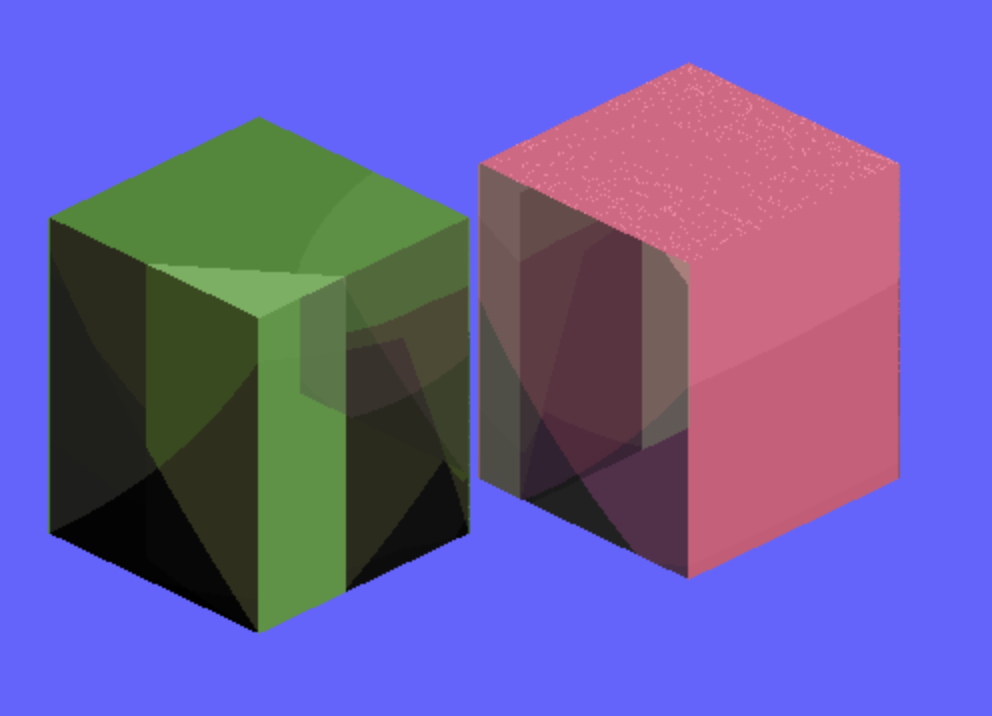
\includegraphics[width=0.5\textwidth]{img/tracing.png}
	\caption{Затенение с помощью трассировки лучей.}
	\label{img:tracing}
\end{figure}

\begin{figure}[H]
	\centering
	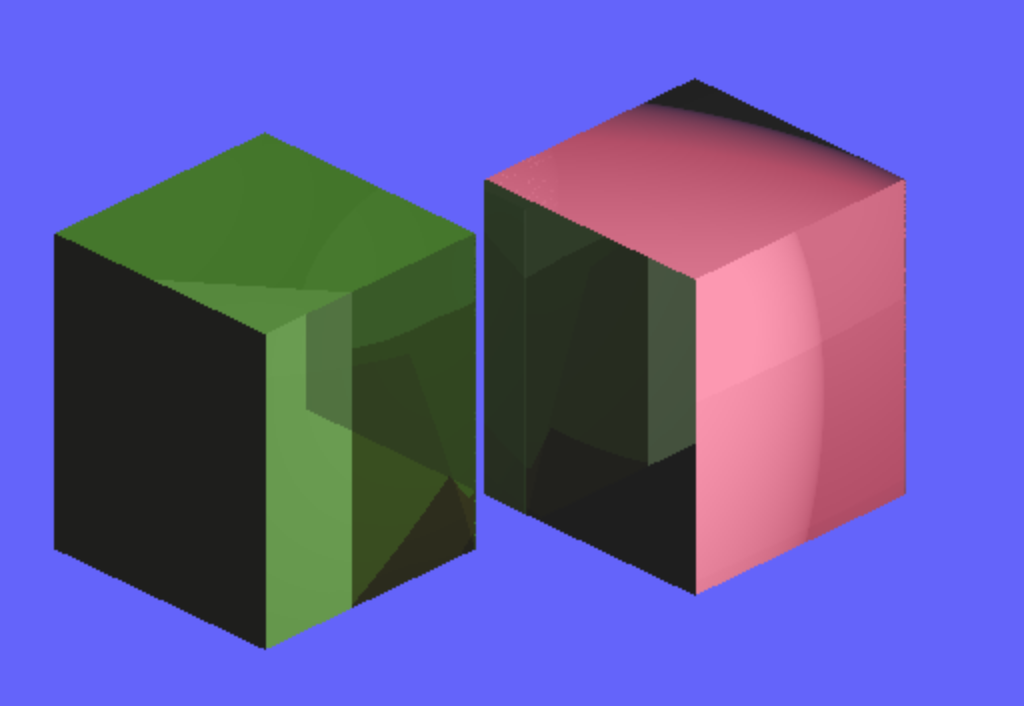
\includegraphics[width=0.5\textwidth]{img/fong.png}
	\caption{Затенение с помощью модели Фонга.}
	\label{img:fong}
\end{figure}

Был проведён опрос 10 человек с целью выяснить субъективные различия между
результатами затенения.
В результате выяснено, что отличия следующие:
\begin{itemize}
    \item
        модель Фонга дала наименьшую яркость,
        а метод отражательных карт теней -- наибольшую;
    \item тени, полученные в методом Фонга, неоднородны;
    \item
        в результате трассировки лучей есть области тени,
        причина возникновения которых не ясна;
    \item
        в результате метода отражательной карты теней
        не все части объектов освещены,
        что объясняется конечными размерами карты теней.
\end{itemize}

\section{Исследование времени затенения}
Проведено исследование времени работы программы.
При расчёте среднего значения производилось 5 замеров.
В процессе измерении времени ноутбук был включен в сеть электропитания
и был нагружен только системными приложениями.
На рисунках \ref{fig:2obj_2src}--\ref{fig:2obj_1src} представлены зависимости
времени построения квадратного изображения сцены от длины его стороны.

\begin{figure}[H]
	\centering
	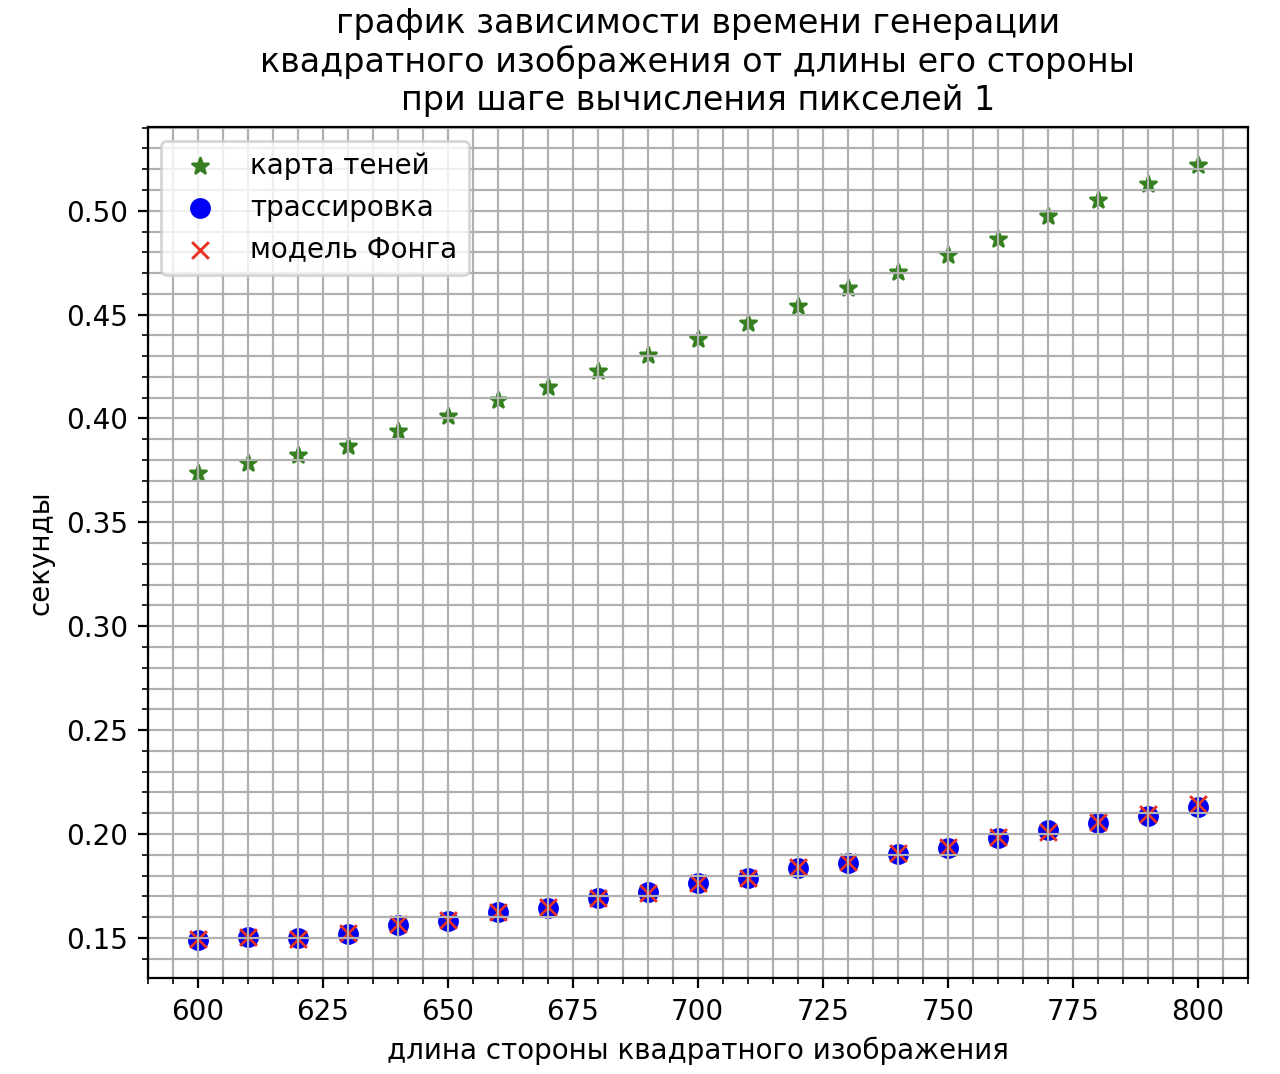
\includegraphics[width=0.65\textwidth]{img/2obj_2src.png}
	\caption{
        График зависимости времени генерации изображения с шагом 1 от его стороны
        для сцены из 2 объектов и 2 источников.
    }
	\label{fig:2obj_2src}
\end{figure}

\begin{figure}[H]
	\centering
	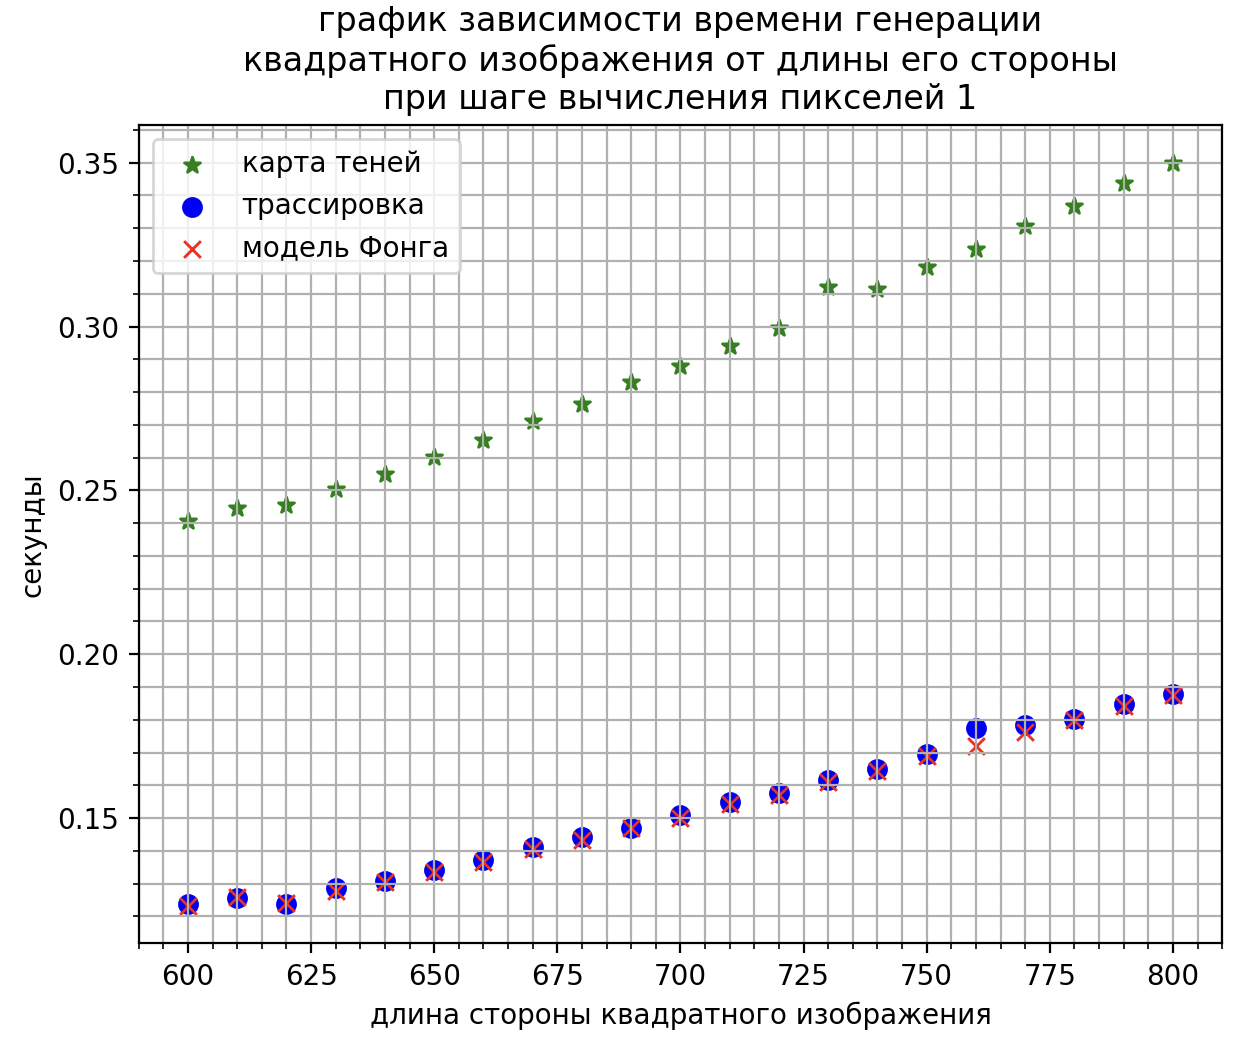
\includegraphics[width=0.65\textwidth]{img/1obj_1src.png}
	\caption{
        График зависимости времени генерации изображения с шагом 1 от его стороны
        для сцены из 1 объекта и 1 источников.
    }
	\label{fig:1obj_1src}
\end{figure}

\begin{figure}[H]
	\centering
	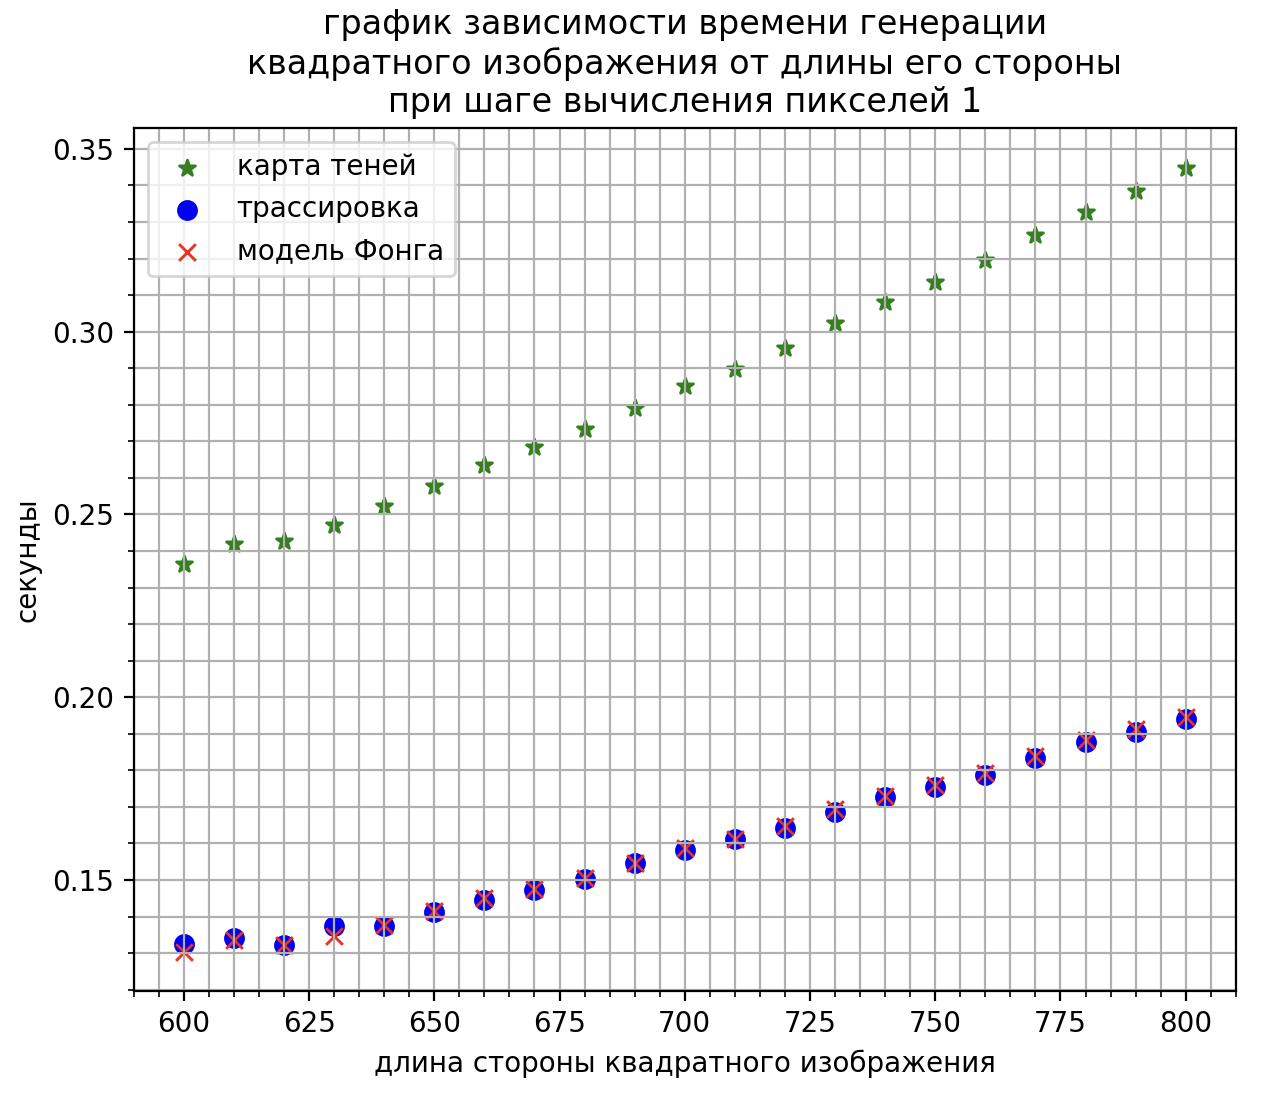
\includegraphics[width=0.65\textwidth]{img/2obj_1src.png}
	\caption{
        График зависимости времени генерации изображения с шагом 1 от его стороны
        для сцены из 2 объектов и 1 источников.
    }
	\label{fig:2obj_1src}
\end{figure}

Из построенных графиков следует, что самая медленная
реализация затенения основана на карте теней.
Реализации моделей освещения, основанных на методах Фонга и трассировки,
наиболее быстрые и тратят на выполнение примерно одинаковое время.
Схожесть их временной эффективности может быть объяснена тем, что обе
модели подразумевают трассировку луча от точки объекта до источника.

\section*{Выводы из технологической части}
В результате данного раздела разработаны и сравнены результаты
3 реализаций методов затенения на примере визуализации сцены.
Также рассчитано среднее время выполнения этих алгоритмов и сравнены
графики зависимостей времени генерации изображения от его размера.
Таким образом, характеристики программного обеспечения исследованы.